\section{Implementering}

\subsection{Model}
Spillets Model består af en række klasser, der tilsammen udgør selve spillets funktioner og objekter. Klassen \textit{Game} er selve spillets logik.

Klassen \textit{Field} bruges til at repræsentere et felt på banen. Den fungerer på samme måde som Javas standard \textit{Point}-klasse. Forskellen mellem \textit{Point} og \textit{Field}, er at vi bruger row og column i stedet for x og y. Spillepladen er delt op i rækker og kolonner, frem for en x- og y-akse. \textit{Field} er lidt mere selvdokumenterende og selve klasse navnet \textit{Point} giver ikke rigtig nogen indikation om hvad det point bruges til. Vores \textit{Field} har også den fordel at man ikke dynamisk kan ændre dens række og kolonne. De er låst fast til den samme værdi og kan kun ændres hvis man opretter et nyt \textit{Field} objekt.

\textit{Food} klassen som repræsentere et stykke mad på banen. \textit{Food} indeholder et \textit{Field} med madens position.

\textit{Food} og \textit{Field} har kun to værdier i sig (en række og søjle). Vi har designet klasserne sådan at de ikke kan ændres efter at de er blevet oprettet. Dette gør at vi kan returnere vores dem i getters og være 100\% sikre på at udefrakommende klasser ikke ændrer dem. Nogen gange kan det godt være svært at resonere omkring kode, hvis alle objekter vilkårligt kan ændre hinanden. Immutable klasser sikre at vi altid kan være sikker på at objekter ikke har ændret sig. Det gør at det er umuligt for Control-pakken at snyde spil logikken.

Slangen er defineret i \textit{Snake}. Slangens krop består af en række felter, hvoraf det første er hovedet, og de resterende er kroppen inklusiv halen som er til sidst. Koordinaterne for disse felter er gemt i en ArrayList. Det første element er slangens første led, hovedet, det andet element er slangens andet led osv. Når slangen bevæger sig tilføjer vi et nyt hoved i listen og sletter halen. Hvis slangen bevæger sig og samtidig spiser noget \textit{Food}, så lader vi være med at slette halen. Slangen vil altid være forholdsvis lille, så om vi gemmer dens elementer i for eksempel en ArrayList eller LinkedList er stort set lige meget. I \textit{Snake} konstruktøren bliver slangens hoved og hale oprettet. Hovedet bliver placeret i banens centrum. Halen placeres i kolonnen til højre for på samme hovedets række.

Vi har valgt at oprette spillepladen i \textit{Game}-klassen som et \textit{Dimension} objekt. Vi bruger ikke en \textit{Board}-klasse, der beskriver banen for sig selv. I bagklogskabens øje burde vi nok have brugt en \textit{Board} klasse. De andre spilelementer er defineret i deres egne klasser for eksempel \textit{Food} og \textit{Snake}.

Slangens flyttes ved at kalde dens \textit{move} metode. Metoden signalere internt til moder \textit{Game} objektet at slangen har bevæget sig. Det gøres med package private metoden \textit{snakeHasMoved(Move)}. \textit{Move} er et enum som betegner slangens handling. Om slangen ikke kan bevæge sig, spiser et æble, er død eller bevæger sig er henholdsvis \textit{EAT\_NECK, EAT\_FOOD, EAT\_BODY} og \textit{NORMAL}. Først tjekkes at slangen ikke bevæger sig ind i dens hals. Hvis det sker signaleres \textit{EAT\_NECK} og der returneres. Det undersøges derefter om der er mad på samme felt som slange hovedets nye placering. Er dette tilfældet, signaleres \textit{EAT\_FOOD}, slangens hoved flyttes og der returneres. Hvis ikke, undersøges der om den nye placering indeholder slangens krop. Gør der det signaleres \textit{EAT\_BODY} og returneres. Hvis ikke, flyttes slangens hoved til den nye position og halen i slangen fjernes. Resten af slangens krop følger med, da slangens ArrayList automatisk skifter hvert index, når den ny hoved placering indsætte som det første element.

I \textit{Game} klassen findes \textit{snakeHasMoved(Action)} metoden, som \textit{move} bruger til at signalere med. Den sætter vundet eller tabt tilstanden i spillet og tjekker om slangen har spist. Hvis den har spist oprettes et nyt mad objekt. Den inkrementerer også scoren. 

Herudover findes \textit{generateFood} metoden, som sikrer generere et nyt stykke mad, på et gyldigt felt, dvs. et felt der ikke er udfyldt af slangen. For at sikre dette, placeres æblet på et tilfældigt felt inden for banens rammer, hvorefter der undersøges om et af slangens led har samme koordinater som æblets felt. Er dette tilfældet, gives æblet et nyt felt, indtil det lander på et felt uden slangen. Er slangen tilpas stor, er dette dog ikke effektivt, da der er stor sandsynlighed for at ramme et felt, der er optaget af slangen. Af denne årsag undersøger metoden først, om slangen fylder mere end halvdelen af banen. Er dette tilfældet, laves der i stedet en liste med alle tomme felter vha. en for-løkke, der løber gennem alle række og kolonner, hvorefter et tilfældigt element i listen vælges som æblets position.

Klasser \textit{Game} nedarver fra klassen \textit{Observable}, så det er muligt for View at modtage ændringerne i Model, uden at Control skal signalere til View at den har ændret Model.

\subsubsection{Immutable Model klasser}
Klasserne \textit{Food} og \textit{Field} er meget små. De har kun to værdier i sig (en række og søjle). Vi har designet klasserne sådan at de ikke kan ændres efter at de er blevet oprettet. Dette sikre os at vi kan returnere vores dem i getters og være 100\% sikre på at udefrakommende klasser ikke ændrer dem. Nogen gange kan det godt være svært at resonere omkring kode, hvis alle objekter vilkårligt kan ændre hinanden. Immutable klasser sikre at man altid kan være sikker på at objekter ikke har ændret sig. Det gør at det er umuligt for Control-pakken at snyde spil logikken.


\subsection{View (Brugergrænsefladen)}
Brugerfladen er samlet i klassen \textit{View} der forlænger \textit{JFrame}. I \textit{View} findes en konstruktør, hvor der oprettes et \textit{ScorePanel} objekt og et \textit{BoardPanel} objekt. Der begge er nedarvet fra \textit{JPanel}. \textit{ScorePanel} fylder det øverste af vinduet og \textit{BoardPanel} resten. Boardpanelet viser spil banen med slangen og maden. Slangen og maden er begge firkanter i forskellige farver.

\textit{ScorePanel} klassen forlænger \textit{JPanel} og implementerer \textit{Observer}. Klassen har en \textit{update}-metode, som signalere at panelet skal optegnes på ny. Hver gang noget i spillet ændre kaldes denne function. Metoden \textit{paintComponent} benyttes til at tegne score teksten.

\textit{BoardPanel} forlænger \textit{JPanel} og implementerer \textit{Observer}. \textit{BoardPanel} består af en række draw-metoder, samt en overridet \textit{paintComponent} metode, der kalder draw metoderne for at tegne alle spillets komponenter. I \textit{drawSnake}-metoden bruges positionerne for slangens felter til at tegne slangen. Størrelsen for et felt udregnes i \textit{getWindowRectangle}, og afhænger af vinduets størrelse og antallet af banens felter. Når feltets størrelse er udregnet, tegnes et rektangel i vinduets grafik kontekst. 

Da spillepladen skal være mellem 5x5 og 100x100 felter, kan det skabe problemer, hvis man ikke kan justere størrelsen på vinduet. Vinduet kan være for stort til at passe på en gennemsnitlig computerskærm. Det er derfor nødvendigt at gøre spillets vinduestørrelse fleksibel. En løsning på dette problem ville være at bestemme en fast størrelse for felterne, og lade vinduet justere sin størrelse efter dette. Ulempen ved metoden er, at store baner kan blive for store til at være på en normal skærm. Derfor har vi valgt at lave en fleksibel størrelse for felterne, så de følger forholdet mellem vinduestørrelse og antal felter.
I \figref{udstrukne_felter} kan man se, at hvis vinduet skal være justerbart, så kan man risikere at selve banen bliver aflang og ikke særlig pæn at spille på.

\begin{figure}
	\centering
	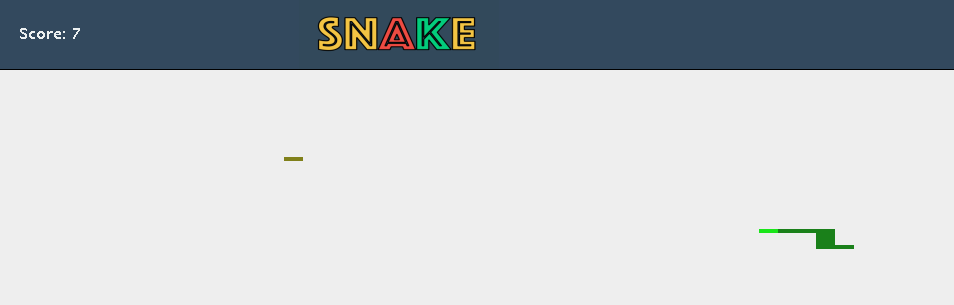
\includegraphics[width=1.0\textwidth]{grundlaeggende/udstrukne_felter.png}
	\caption{\figlab{udstrukne_felter}Eksempel på udstukne felter.}
\end{figure}

\subsection{Control (Styring)}
I Simpel Snake er der ikke brug for nogen menu, og det er derfor muligt at holde styringen af spillet meget simpel. Vi lader \textit{Control} klassen nedarve fra Javas \textit{KeyAdapter}. I dens konstruktør sætter vi den til at lytte efter efter key events på vores \textit{View} klasse.
